% Rule sheet for primes game
% Game design: Grant Sinclair
% Graphic design: Harald Bögeholz

\documentclass{article}

\usepackage{graphicx}
\usepackage{adjustbox}

\newcommand{\card}[1]{\adjustbox{valign=m}{\includegraphics[page=#1, width=2cm]{primecards-screen.pdf}}}
\newcommand{\square}[1]{\adjustbox{valign=m}{
\includegraphics[page=#1, width=2cm]{boardsquares.pdf}}}

\begin{document}


\section*{Setup}

Place the meeples on the starting square. If there are

\begin{description}

\item[2 players:] 3 meeples per player

\item[3 players:] 2 meeples per player

\item[4--6 players:] 1 meeple per player

\end{description}

Shuffle the deck and put it onto the drawpile with the black side up. Cut the deck and deal one card to each player.

\section*{Gameplay}

The players take turns in a clockwise direction. On their turn, a player may \textbf{trip} an opponent by playing any number of their cards white side up so that the symbols exactly match the symbols on the square occupied by the opponent. The opponent meeple(s) are moved back by the sum of the numbers on the cards played. The player may continue tripping opponents as long as they can. After that, the player may \textbf{run} once by playing any number of their cards \textit{with the same number} black side up. A player may choose to pass by neither tripping nor running.

For each opponent meeple tripped and for the run, the player may then move forward one of their own meeples by the sum of the numbers on the cards. Meeples can not be moved beyond 100; if a meeple is too close to 100 and the number is too large, it has to stay in place. You can only reach 100 by playing exactly the right number.

At the end of their turn, the player draws one more card than they played and puts all played cards in the discard pile. When the draw pile runs out, it is not reshuffled; players just stop drawing.

\section*{Example turn}

Let's say on a player's turn there is one opponent meeple on square \square{12} and one opponent meeple on square~\square{5}.

The player trips by playing \card{91} \card{69} for a total of 7, taking one opponent meeple from \square{12} back to \square{5}.

The player now trips again by playing \card{125}, sending \textbf{two} opponent meeples back from \square{5} to the starting square.

Finally, the player \textbf{runs} by playing \card{170}~\card{170}.

The player may now make four moves: 7 for the first trip, 6 and 6 again for tripping two opponents, and finally 16 for the run. They draw six cards (because they played five) and discard the cards from play.

\section*{End of the game}

The game ends when a player gets \textbf{all} their meeples to 100 or when all players pass on consecutive turns. The winner is the player whose \textbf{last} meeple is furthest ahead.

\end{document}
